\begin{figure}[htbp]
\centering
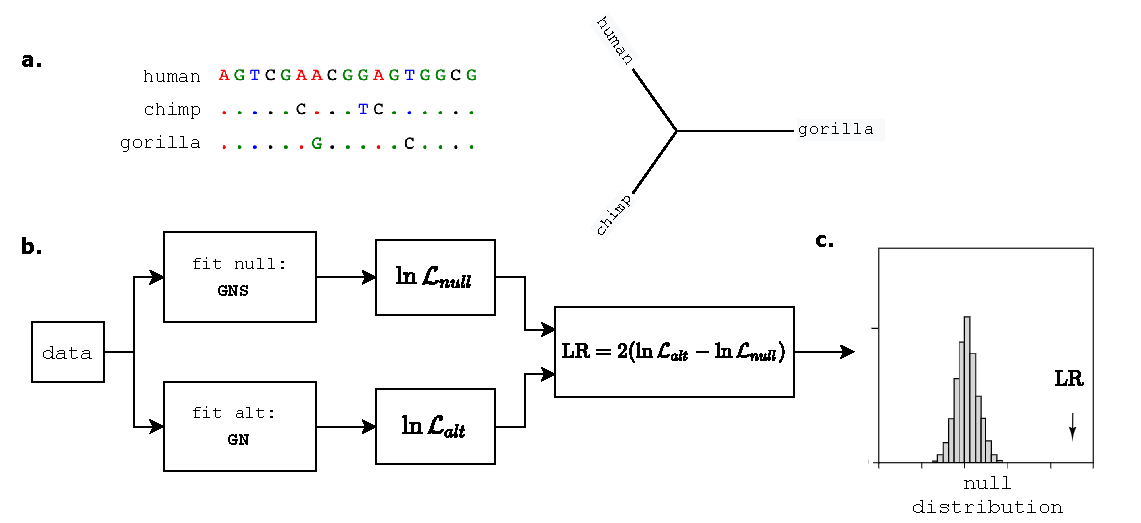
\includegraphics[width=\textwidth]{figures/diagrams/LRT.pdf}
\caption[Likelihood Ratio Test]{\textbf{Likelihood Ratio Test.} \textbf{a}, The data: an alignment of orthologous sequences for human, chimp and gorilla, and a phylogenetic tree indicating the relationship between taxa. \textbf{b}, A LRT comparing substitution models, GNS is the null and GN is the alternate. The log-likelihood ($\ln\mathcal{L}$) for each model is obtained via fitting. The likelihood ratio (LR), is the ratio of the $\ln\mathcal{L}$ of the two models. \textbf{c}, the LR statistic is compared to the null distribution. In this case the statistic exceeds the distribution of values we would expect if the null was true, we would thus conclude that process is described significantly better with the alternate (GN) process.}
\label{fig:lrt}
\end{figure}